\section{Introduction}\label{sec:intro}
% Problem, importantness, and specific question
Reward is a fundamental brain function that shapes our behavior through reward-based learning, or reinforcement learning (RL). Positive rewards encourage us to eat food and find mating partners, while negative rewards, such as pain and fatigue, help us protect ourselves. However, regardless of its importance to animal lives, the evolutionary process of such a reward system is underexplored. Reward signals should have evolved to help animals survive and reproduce offspring (e.g., by~\cite{schultzNeuronalRewardDecision2015}), but what kind of environmental conditions have influenced the evolution of varieties of rewards remains unclear.

\begin{figure}[t]
  \centering{}
  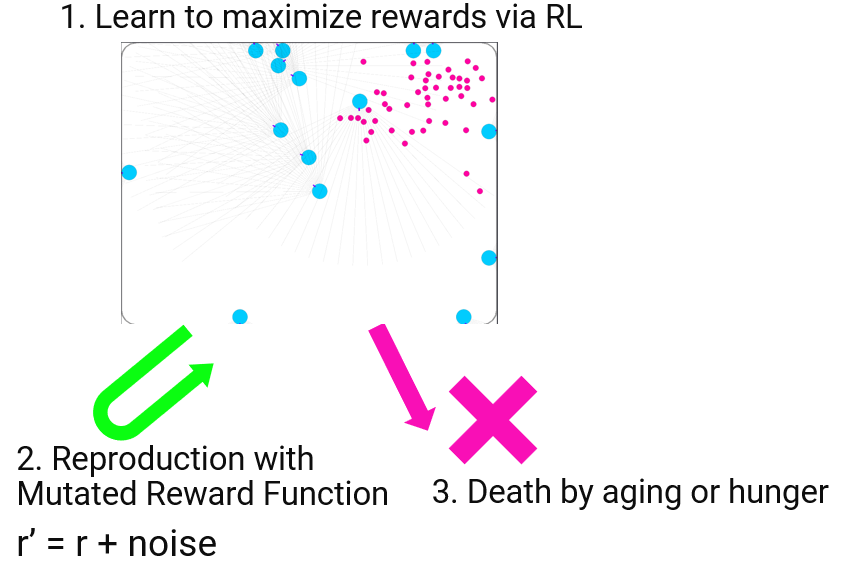
\includegraphics[width=6cm]{emevo-scheme-min.png}
  \caption{
    A schematic figure on our evolutionary framework.
    Aagens learn to maximize their reward functions inherited from their parents.
    They reproduce children with mutated reward functions and die from aging or hunger.
  }\label{figure:scheme}
\end{figure}

% What we do
While biological studies in evolution are important, the difficulty of observing reward evolution in real animals motivates us to use artificial evolutionary simulation. Hence, we conduct an evolutionary simulation of RL agents to examine how different environmental conditions lead to different rewards. Each agent inherits a reward function from its parent and learns to get more rewards by RL during its lifetime. Contrary to previous studies on the evolution of learning \citep{hintonHowLearningCan1987,singhWhereRewardsCome2009} with centralized selection strategies, we design a distributed evolutionary model inspired by embodied evolution (EE) framework \citep{watsonEmbodiedEvolutionDistributing2002,bredecheEmbodiedEvolutionCollective2018}. In our model, birth and death for agents are evaluated independently based on their age and internal energy level, allowing the population change. With this approach, we expect rewards contributing to population growth to be selected. We show a schematic figure on our evolutionary framework in \cref{figure:scheme}.

% Foraging environment
% Simulation
We implement our distributed evolution framework in a simple virtual environment where agents need to hunt foods to live longer and produce children based on 2D physics simulation. In this environment, we let agents evolve simple reward functions that map food intake and the magnitude of motor output to a scalar, which we expect to correspond to food pleasure and fatigue. Our results show that biologically reasonable reward functions evolve from randomly initialized ones given sufficient learning ability. We then find that metabolic balance, food density, and food relocation influence the shape of the reward function. Furthermore, we examine the evolution of rewards for poor and poisonous rewards. Our results show a more unstable evolution of rewards for such less important foods, sometimes leading to speciation.

\section{Preliminaries and Related Works}\label{sec:related}
We follow the standard computational RL framework \citep{suttonReinforcementLearningIntroduction2018} based on the Markov decision process (MDP). MDP $\M{}$ consists of a tuple $(\X{}, \A{}, p, r, \gamma)$, where $\X{}$ is reward function, and $\gamma \in [0, 1]$ is the discount factor. A standard objective in MDP is the discounted cumulative return $G \defequal{} \sum_{t=0}^{\infty}\gamma^t R_{t}$, where $R_t$ is the reward received at time $t$. An RL agent has policy $\pi: \X \times \A \rightarrow [0, 1]$ and seeks to find the the optimal policy $\pi^{*}$ that maximizes $\E \left[G|\pi\right]$. The state-value function $V^\pi(s) \defequal \sum_{a \in \A} \pi(a|s) \left( r(s, a) + \gamma \sum_{s' \in \X} P(s'|s, a) V^\pi(s') \right)$ is often used in RL algorithms. Observation $o \in \Omega~(\Omega \subseteq \X)$ refers to a part of the state that an agent can observe.

Our reward model is inspired by the neuroscience of reward system \citep{schultzNeuronalRewardDecision2015, berridgePleasureSystemsBrain2015}. Notably, \citet{berridgeDissectingComponentsReward2009} argue that the brain reward system consists of three independent components: liking, wanting, and learning. In analogy with computational RL, liking corresponds to reward function, wanting corresponds to learned policy, and learning corresponds to learning state value $V$.

While there were previous attempts to evolve rewards in a single-agent setting \citep{singhWhereRewardsCome2009,niekumEvolutionRewardFunctions2011,zhengWhatCanLearned2020},
%While evolutionary robotics studies \citep{nolfiEvolutionaryRoboticsBiology2004} often employ a centralized selection scheme similar to genetic algorithm \citep{mitchellIntroductionGeneticAlgorithms1998},
%where highly evaluated elites are selected as parents. On the contrary,
we employ a distributed embodied evolution (EE) framework \citep{watsonEmbodiedEvolutionDistributing2002,bredecheEmbodiedEvolutionCollective2018}
%that employs a decentralized evolution without centralized evaluation
where agents evolve locally following birth and death rules. This method has the advantage that the evaluation of genetic traits depends on population dynamics, which is more natural.

Our work is inspired by the series of studies \citep{elfwingBiologicallyInspiredEmbodied2005,elfwingDarwinianEmbodiedEvolution2011,elfwingEmergencePolymorphicMating2014}, which tried to evolve parameters related to RL through EE framework. Notably, \citet{elfwingDarwinianEmbodiedEvolution2011} evolved supplementary sharing rewards and parameters of RL agents.
Inspired by these works, we attempt to evolve the entire reward functions in our experiments.

\section{Simulation Model and Environment}\label{sec:method}

\begin{figure}[t]
  \centering{}
  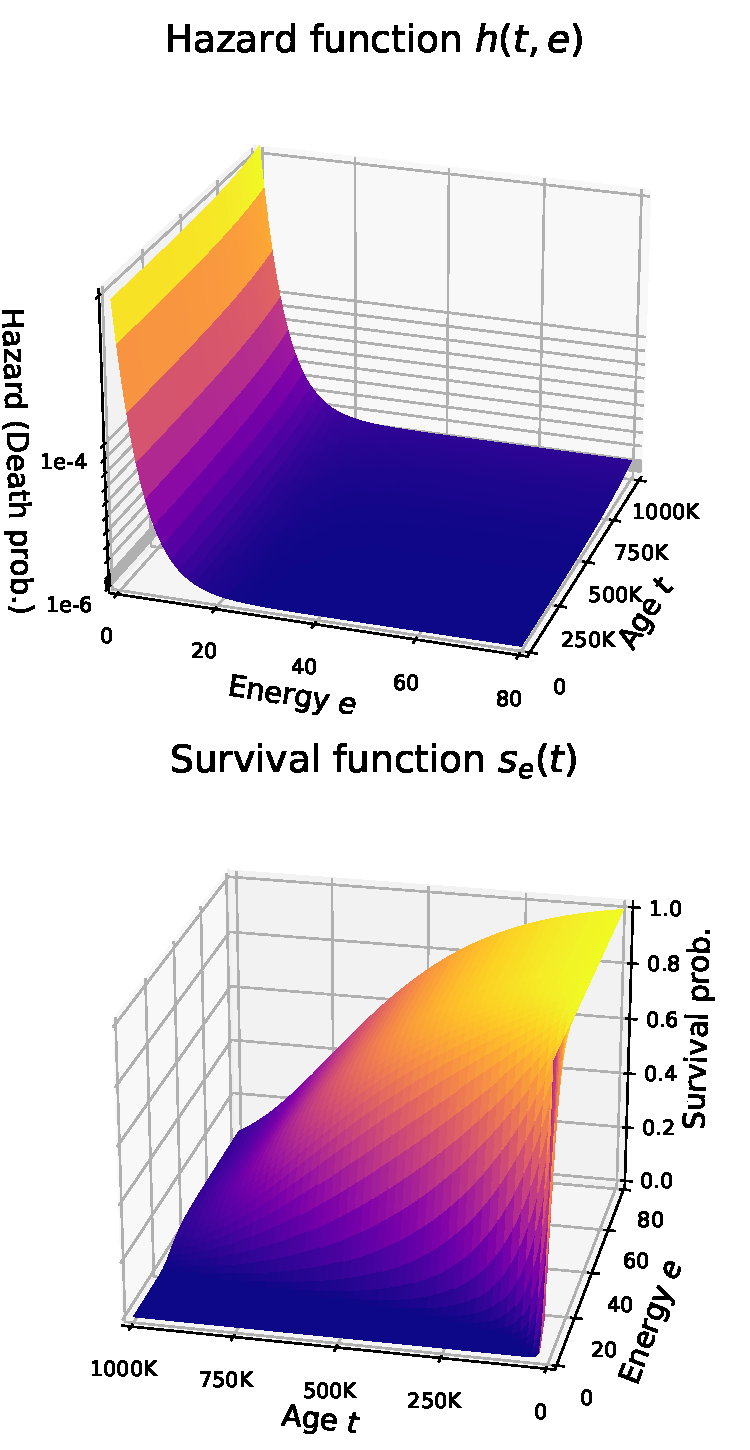
\includegraphics[width=6cm]{hazard_and_survival.pdf}
  \caption{
    \textbf{Upper:} Hazard function $h(t)$ used in our experiments.
    \textbf{Lower:} Survival function $S(t)$ corresponding to the hazard function above.
  }\label{figure:hs}
\end{figure}

\paragraph{Energy-based death and birth model}
We employ an energy-based metabolic model similar to \citet{hamonEcoevolutionaryDynamicsNonepisodic2023}. Each agent maintains their energy level $e$, which increases by eating food and decreases by the basal metabolism and taking a motor action.
The mortality of the agent with energy level $e$ and age $t$ is modeled by the hazard function:
\begin{align}
  h(t, e) = \frac{\kappa_{h}}{1 + \alpha_{e}\exp(\beta_{he}e)} + \alpha_{t} \exp(\beta_{ht} t).
  \label{eq:h}
\end{align}
The first term in \cref{eq:h} increases as energy levels decrease following a sigmoidal curve where $\kappa_{h}$ is the scale, $\beta_{he}$ is the slope, and $\alpha_{e}$ defines the shape when $e=0$. The latter term increases exponentially as the agent ages with the cale $\alpha_{t}$ and the slope $\beta_{ht}$, called Gompertz hazard model \citep{gompertzXXIVNatureFunction1825,kirkwoodDecipheringDeathCommentary2015}.
We show the shape of $h$ with parameters used in our experiments in the upper panel in \cref{figure:hs}. The lower panel in \Cref{figure:hs} shows the survival function $s_{e}(t) = \exp (-\int_{0}^{t}(h(t, e)) dt)$ corresponding to $h$, which is the probability for an agent to survive to the age $t$ under the assumption that it keeps the same energy level $e$. We can see that the survival probability more sharply decays with aging when the energy level is low.

\begin{figure}[t]
  \centering{}
  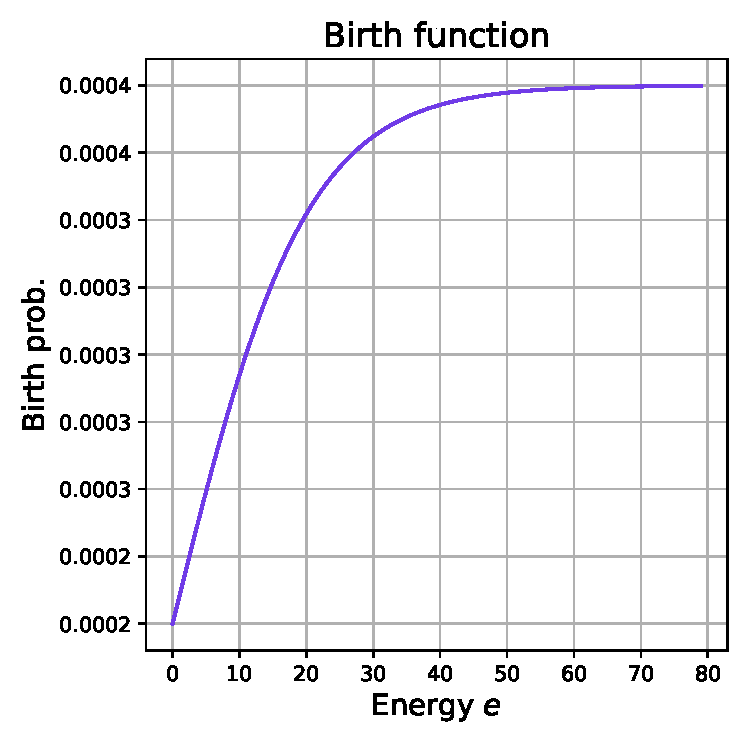
\includegraphics[width=6cm]{birth.pdf}
  \caption{Birth function $b(e)$ used in our experiments.}\label{figure:birth}
\end{figure}

\begin{table}[t]
  \begin{subtable}[h]{0.45\columnwidth}
    \centering
    \begin{tabular}{cc}
      \toprule
      Parameter & Value \\
      \midrule
      $\kappa_{h}$ & 0.01 \\
      $\alpha_{e}$ & 0.02 \\
      $\beta_{he}$ & 0.2 \\
      $\alpha_{ht}$ & \num{2e-7} \\
      $\beta_{t}$ & \num{4e-6} \\
      \bottomrule
    \end{tabular}
  \end{subtable}
  \begin{subtable}[h]{0.45\columnwidth}
    \centering
    \begin{tabular}{cc}
      \toprule
      Parameter & Value \\
      \midrule
      $\kappa_{b}$ & \num{4e-4} \\
      $\beta_{b}$ & 0.1 \\
      \bottomrule
    \end{tabular}
  \end{subtable}
  \caption{Parameters of $h$ (left) and $b$ (right) used in our experiments.}\label{table:hb}
\end{table}

For simplicity, we employ an asexual reproduction model with the birth function, the probability for an agent with energy level $e$ to produce a child in a time step:
\begin{align}
 b(e) &= \frac{\kappa_{b}}{1 + \exp(\beta_{b}e)}.
 \label{eq:b}
\end{align}
The birth rate $b(e)$ increases with $e$ following a sigmoidal curve where $\kappa_{b}$ is the scale and $\beta_{b}$ is the slope.
\Cref{figure:birth} shows the shape of $b$ for the parameters used in our experiments. We show all paramters of $h$ and $b$ in \cref{table:hb}. With this choice of parameters, we expect the maximum lifetime of an agent to be around \num{1e6} steps.

\paragraph{Environment}

\begin{figure}[t]
  \centering
  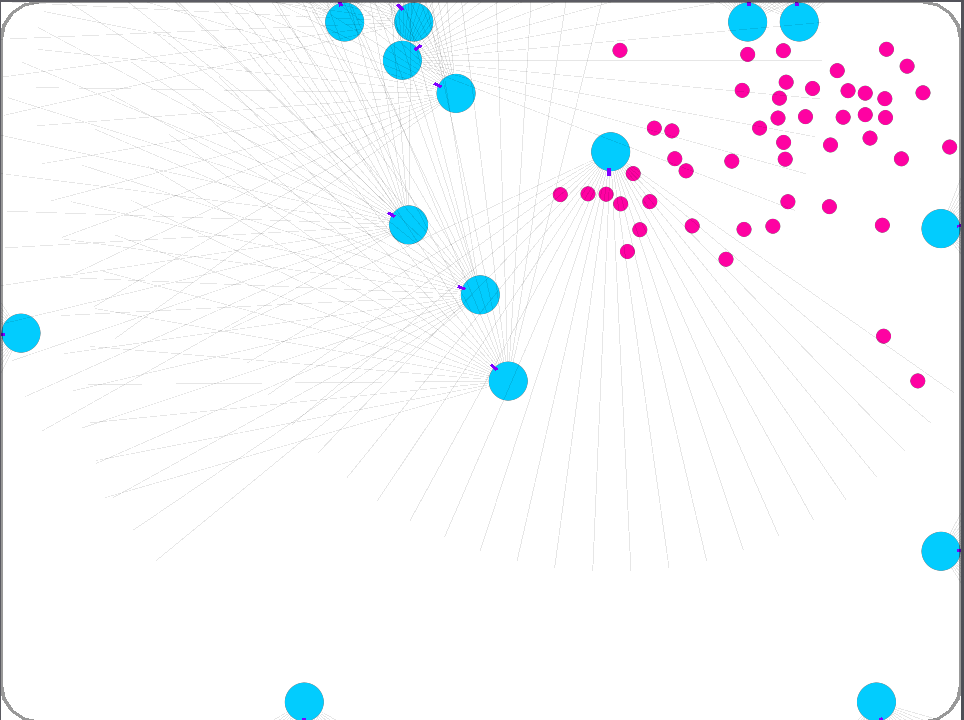
\includegraphics[width=6cm]{emevo-ss.png}
  \caption{
    Simulation environment used in our experiments.
    Blue circles are agents, red circles are foods, and outer gray lines are walls.
    Thin gray lines around agents indicate distance sensors.
  }\label{figure:env}
\end{figure}

\begin{figure}[t]
  \begin{subfigure}[t]{4cm}
    \centering
    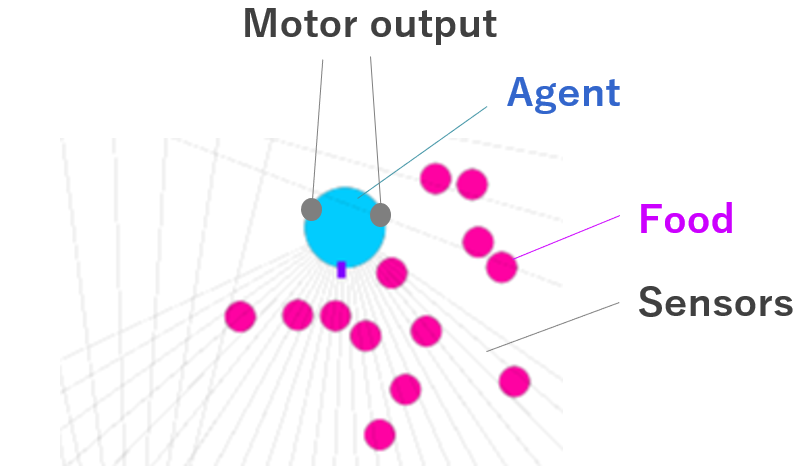
\includegraphics[width=4cm]{emevo-anno.png}
  \end{subfigure}
  \begin{subfigure}[t]{4cm}
    \centering
    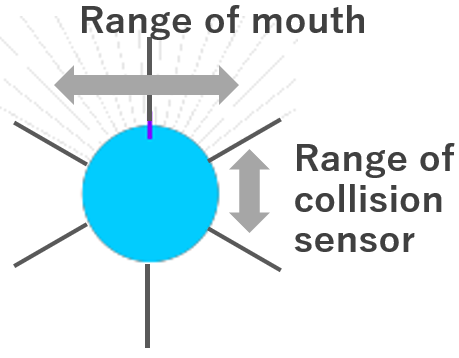
\includegraphics[width=4cm]{emevo-mouth.png}
  \end{subfigure}
  \caption{
    Description of the environment.
    The left figure shows an agent, foods, distance sensors, and the positions of motor outputs.
    The right figure shows the ranges of an agent's mouth and each collision sensor.
  }\label{figure:env-discr}
\end{figure}

We designed a continuous 2D environment shown in \cref{figure:env}. Blue circles indicate agents and red circles indicate foods. The environment is implemented by a 2D rigid-body physics simulation. Agents can move by producing driving forces on the left and right sides of the body, as shown in \cref{figure:env-discr}. An agent has multiple range sensors in its front, which can sense the type and the distance to the closest object within $120$ degree. Sensible objects include foods, other agents, and walls. They can also sense the collision with each object and the approximate location of the collision with a resolution of $60$ degree, as shown in \cref{figure:env-discr}.

% This eat-driven emergence is not consistent with the growth model below. Better report the actual food-producing process rather than theoretical approximation.
The agent can eat food by touching it and gain energy $e_{\mathrm{food}}$. We use $e_{\mathrm{food}} = 1$ in our experiments. In experiments with less nutrient-poor or poisonous foods, they have different energy gain $e_{\mathrm{poor}} = 0.2$ and $e_{\mathrm{poison}} = -0.4$. After foods are eaten, they are regenerated in a random place. To regulate the rate of food regeneration, we maintain the internal food number $n_{t}$ at time $t$ which follows a logistic growth function: $n_{t + 1} = n_{t} + gn_{t}(1 - \frac{n_{t}}{n_{\mathrm{max}}}) - n_{t}^{\mathrm{eaten}}$, where $g$ is the growth rate, $n_{\mathrm{max}}$ is the capacity of food, and $n_{t}^{\mathrm{eaten}}$ is the number of eaten foods at time $t$. Food is regenerated when the integer part of $n^{t}$ is more than the actual number of foods in the environment. We use $n_{\mathrm{max}} = 50$ and $g = 0.01$ in our experimens.

The agent consumes energy via active and basic metabolism. At each step $t$, An agent $i$ losts energy $e_{\mathrm{act}} |a_{t}^{i}|$, where $|a_{t}^{i}|$ is the Euclid norm of the agent's motor output $a_{t}^{i}$ and $e_{\mathrm{act}}$ is a scaling coefficient. In addition, it also consumes energy $e_{\mathrm{basic}}$ at every step. In our experiments, we use $e_{\mathrm{act}} = \num{2e-5}$ and $e_{\mathrm{basic}} = 0.001$, leading to the consumption of $0.002 \sim 0.003$ energy by one step. It means that agents need to eat food at least once in $500$ or $1000$ steps to maintain their energy level.

When an agent makes a child, a new agent is placed in a random location sampled from a Gaussian distribution centered around its parent. Reproduction fails when all $10$ sampled locations are not available. The child inherits a proportion of the parent's energy $\eta e \in [0, 1]$, and the parent's energy level decreases to $(1-\eta)e$, where $\eta \in [0, 1]$ is the ratio of energy sharing. We used $\eta = 0.4$ in our experiments. The child also inherits its reward function from the parent with some mutation.

Since we need to maintain agents for evolution, the multi-agent interaction can be a huge bottleneck in our simulation. To overcome this challenge, we implement our environment using JAX Python library \citep{jax2018github} so that the entire simulation loop is executed on GPU. Inspired by recent works on 3D rigid body physics simulation using JAX (e.g., \citet{brax2021github} and MuJoCo \citep{todorov2012mujoco} MJX\footnote{\url{https://mujoco.readthedocs.io/en/stable/mjx.html}}), we implement our 2D physics engine using JAX and build our
environment on top of that, optimizing it for multi-agent setting. Our simulator implements projected Gauss-Seidel method with position correction \citep{catto2005iterative} that is pretty common in 2D game physics engines such as Box2D\footnote{\url{https://box2d.org}} and Chipmunk\footnote{\url{https://chipmunk-physics.net}}.

\paragraph{Reward Function with Evolving Weights}
We assume that the reward function is determined at birth with mutation and does not change during the agent's lifetime. We use food intake and the magnitude of the agent's action (motor output) as inputs to the reward function. We expect a positive food reward to evolve to acquire energy and a negative reward for action to evolve to save energy.
We model the reward of an agent $i$ at time $t$ by $r^{i}_{t} = w_{\mathrm{food}}^{i}n_{t}^{i} + c_\mathrm{act} w_{\mathrm{act}}^{i}|a_{t}^{i}|$, where $n_{t}^{i}$ is the number of foods that the agent at that step. $w_{\mathrm{food}}^{i}$ and $w_{\mathrm{act}}^{i}$ are evolvable reward parameters of an agent $i$. Because an agent gets the action reward at every step but doesn't get the food reward so often, we use a fixed parameter $c_\mathrm{act}$ to scale the reward. We use $c_\mathrm{act}=0.01$ in our experiments. In experiments with poor or poisonous foods, we use another evolvable reward parameter $w_{\mathrm{poor}}^{i}$ or $w_{\mathrm{poison}}^{i}$.
\todo{Cauchy mutation, clip range (-10, 10)}

\begin{table}[!htb]
  \centering
  \caption{RL parameters}\label{tab:rl-param}
  \begin{tabular}{ll}
    \toprule
    Parameter & Value \\
    \midrule
    Discount factor ($\gamma$) & 0.999 \\
    Rollout steps ($N$) & 1024 \\
    Minibatch size & 256 \\
    Number of optimization epochs & 10 \\
    PPO Clipping parameter & 0.2 \\
    Entropy coeff. & 0.0 \\
    GAE parameter ($\gamma$) & 0.95 \\
    Adam learning rate & \num{3e-4} \\
    Adam $\epsilon$ & \num{1e-7} \\
    Size of hidden layer in MLP & 64 \\
    \bottomrule
  \end{tabular}
\end{table}

\paragraph{Reinforcement Learning}
We use Proximal Policy Optimization \citep{schulmanProximalPolicyOptimization2017} as an RL algorithm because of its fast computation time. In addition to the touch and collision sensor inputs in \cref{figure:env-discr}, the agent takes its angle, velocity, and energy level as an observation. The action space is a continuous two-dimensional vector corresponding to the forces applied to the left and right sides of the body. Following the standard practice in the literature, we use a multi-layer perception (MLP) with hyperbolic tangent activation to represent the agent's policy, which is randomly initialized for each newborn. We show RL parameters used in our experiments in \cref{tab:rl-param}.

% Add a line for reward acquisition; after observation or action?
\begin{algorithm}[!htb]
  \caption{Reward evolution with asexual reproduction}\label{alg:reward-evo}
  \begin{tabular}{lll}
    \textbf{Input:} & $Pop$ & Initial population of agents \\
                    & $Env$ & Simulation environment \\
                    & $h, b$ & Hazard and birth functions \\
                    & $m$ & mutation function \\
                    & $N$ & Rollout step used in RL \\
                    & $\eta$ & Energy share ratio
  \end{tabular}
  \begin{algorithmic}[1]
    \Loop{}
    \LComment{Interact with environment}
    \ForAll{$agent \in Pop$}
      \State{$o \gets agent$'s observation in $Env$}
      \State{$a \gets $ sample from $agents$'s policy $\pi_{agent}(\cdot|o)$}
      \Once{in $N$ steps}
        \State{Update $agent$'s policy $\pi_{agent}$ via RL}
      \EndOnce{}
    \EndFor{}
    \State{Step $Env$ using collected actions}
    \State{Update $agent$'s energy level}
    \LComment{Process birth and death}
    \ForAll{$agent \in Pop$ with energy $e$ and age $t$}
      \State{$e \gets e + e_{\mathrm{food}} n_{\mathrm{food}} - e_{\mathrm{act}}|a| - e_{\mathrm{basic}}$}
      \With{Probability $b(e)$} \Comment{Birth}
        \State{$e \gets (1 - \eta) e$}
        \State{$r \gets agent$'s reward function}
        \State{Create a new agent with $\eta e$ and $m(r)$}
      \EndWith{}
      \With{Probability $h(t, e)$} \Comment{Death}
        \State{$agent$ is removed from $Pop$ and $Env$}
      \EndWith{}
    \EndFor{}
  \EndLoop{}
\end{algorithmic}
\end{algorithm}

\paragraph{Simulation Procedure}
We show the pseudocode of our entire simulation procedure in \cref{alg:reward-evo}. Each agent has its innate, immutable reward function and learnable neural network policy. At each step, it observes sensory inputs from the environment and takes action. Once in $N$ steps, the agent updates its policy via RL using the past $N$ step experiences. After environmental interaction, all agents can make a child and die based on the birth function $b$ and hazard function $h$. The new agent inherits a fraction of the parent's energy and mutated reward function.

\section{Results}
As a baseline environment, we use the setting where food is always regenerated in the upper right of the room, as the left figure in \cref{figure:env} shows. All experiments start from $50$ agents with an energy level of $40.0$. Birth and hazard parameters in \cref{table:hb} are tuned so that the population size is around $130\sim 150$ through evolution. Initial reward weights are sampled from a zero-mean Gaussian distribution with a standard deviation of $0.1$, so they should take values close to $0$. We conducted about one hundred thousand steps ($\num{1024e4}$) of the simulation, resulting in $300$ to $400$ generations, which takes $14\sim16$ hours on NVIDIA P100 GPU.

\begin{figure}[!htb]
  \centering
  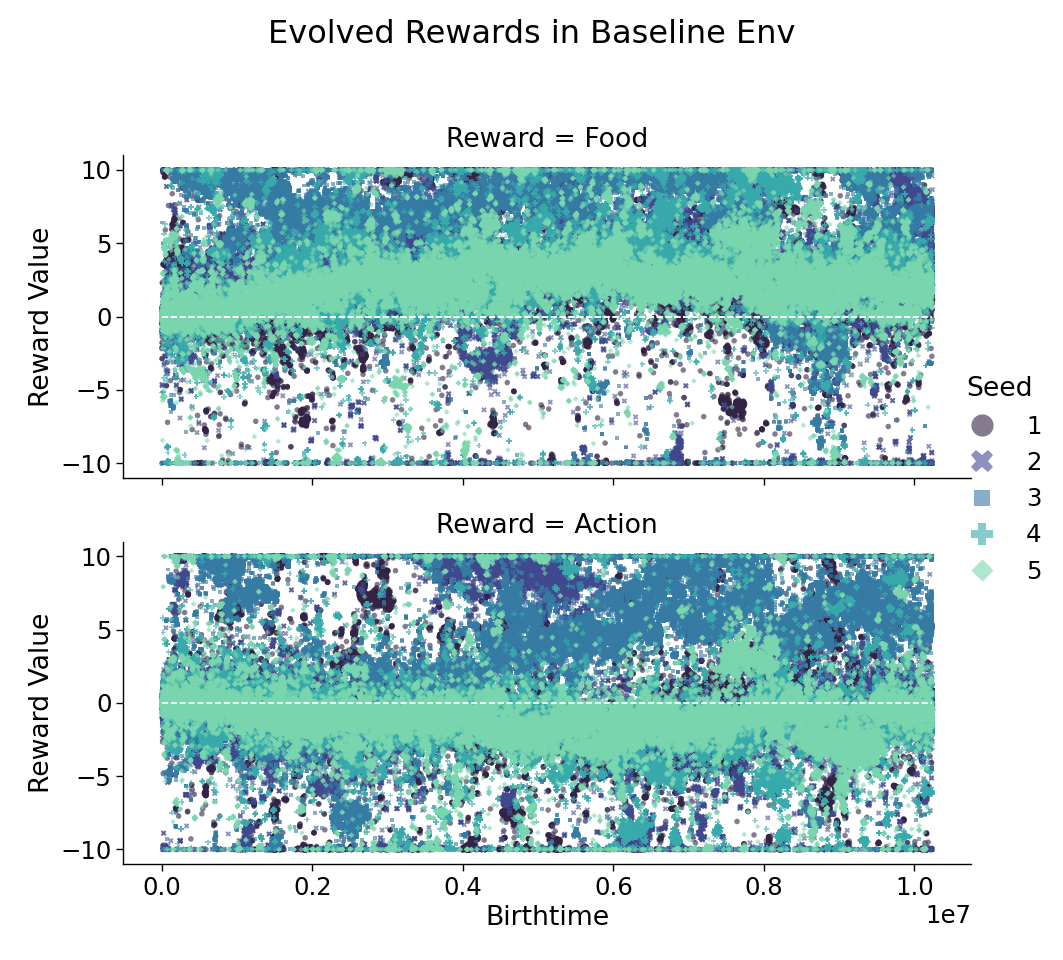
\includegraphics[width=8cm]{baseline-min.png}
  \caption{
    Evolved rewards in the baseline setting.
    The upper figure shows food rewards by agents' birth time, while the lower figure shows the evolution of action rewards.
    Different colors and marker shapes indicate runs with different random seeds.
  }\label{figure:result-baseline}
\end{figure}

\Cref{figure:result-baseline} shows the evolved reward weights with 5 random seeds in the baseline environment. We observe that food reward is positive in all 5 runs, while action reward tends to be negative in most of the runs. Thus, we can say that agents have acquired rewards that contribute to increasing their energy levels through evolution. The only exception is that action reward is largely positive in one random seed, which has a negative impact on the population size. This run has the least average population size of $120.6$ in the last $\num{3e6}$, while it is from $136$ to $149$ in other runs with negative action rewards. This result suggests that such unfavorable reward for population growth can be chosen when there is no competition with other species and sufficient energy resources.

\begin{figure}[!htb]
  \centering
  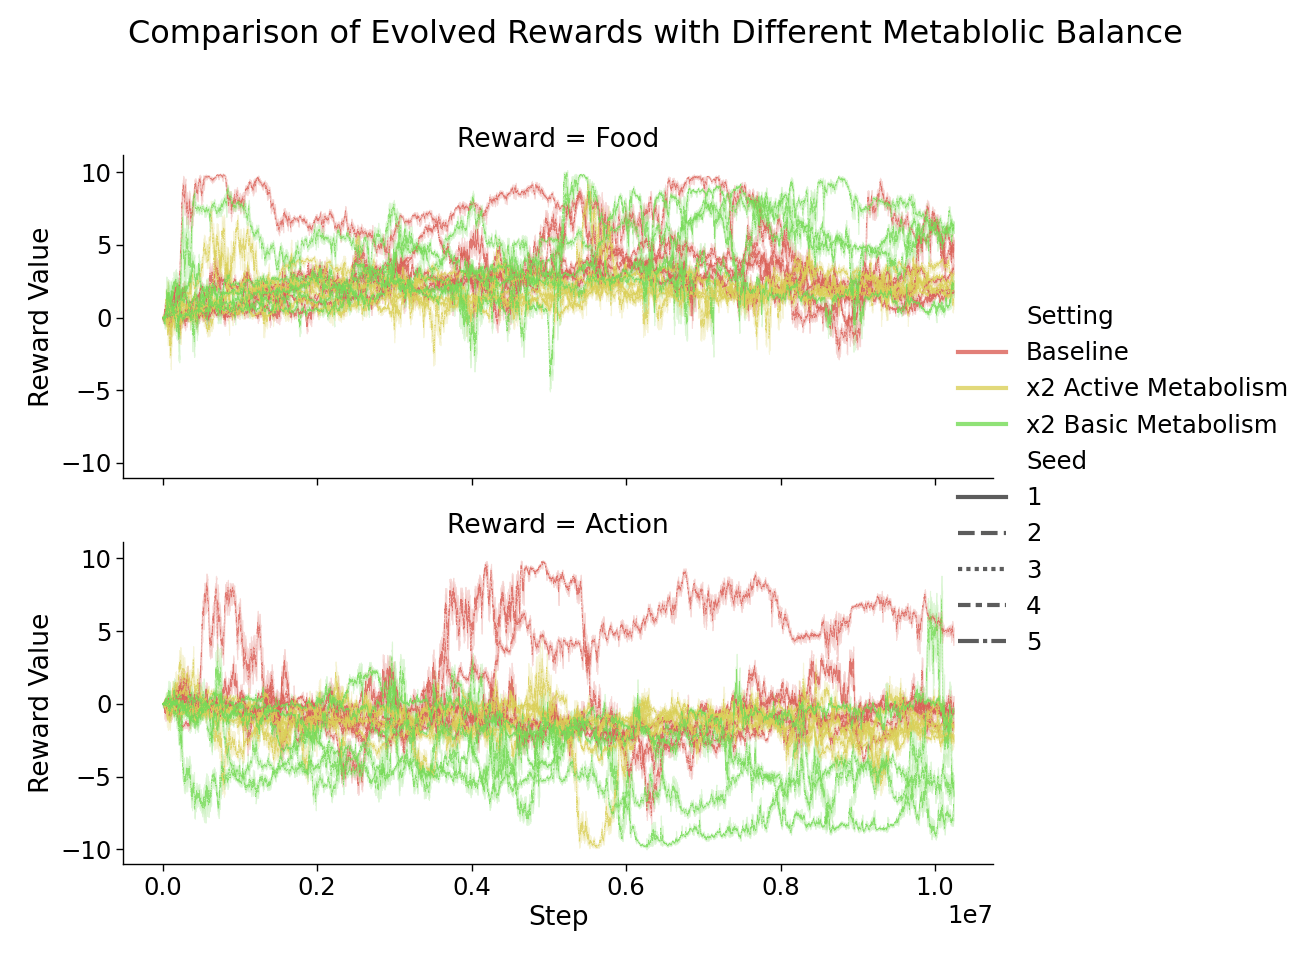
\includegraphics[width=8cm]{comp_metabolism-min.png}
  \caption{
    Comparison of evolved rewards between different metabolic balances.
    Each line shows the reward weight averaged over all agents alive at that time with one random seed, resulting in five lines for each setting.
    Different colors indicate different metabolic balances.
  }\label{figure:result-metabolism}
\end{figure}

\begin{figure}[t]
  \begin{subfigure}[t]{3cm}
    \centering
    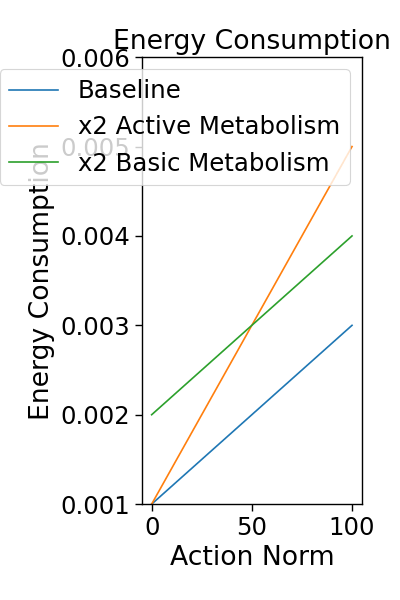
\includegraphics[width=3cm]{energy-consumption-min.png}
  \end{subfigure}
  \begin{subfigure}[t]{5cm}
    \centering
    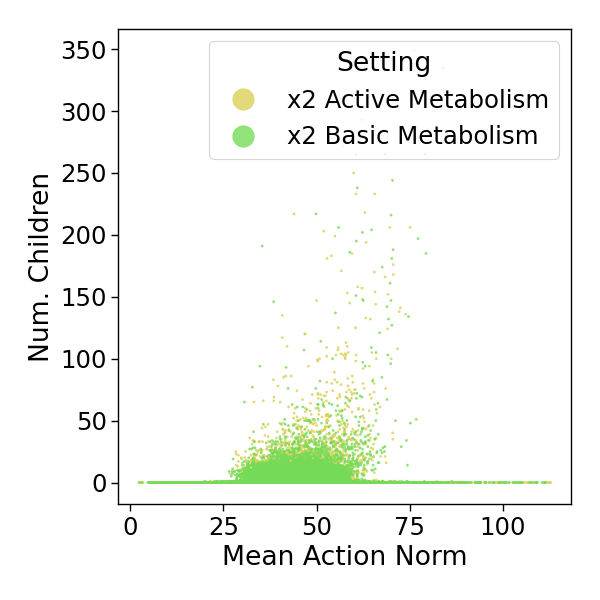
\includegraphics[width=5cm]{metabo-scatter-min.png}
  \end{subfigure}
  \caption{
    \textbf{Left:} Energy consumption per action norm in three settings.
    \textbf{Right:} Relationship between the average of action norm ($|a_{t}^{i}|$) and the number of children.
  }\label{figure:scatter-metabo}
\end{figure}

\paragraph{Effect of Metabolic Balance}
To investigate the effect of metabolic balance on rewards, we run simulations with two different metabolic balances. One has double active metabolism ($e_{\mathrm{act}} = \num{4e-5}$), and the other has double the basic metabolism ($e_{\mathrm{basic}} = 0.002$). Note that parameters are adjusted so that energy consumption by active and basic metabolism is roughly equal in the baseline setting.
\Cref{figure:result-metabolism} compares the results between the baseline, double active metabolism (\texttt{x2 Active Metabolism}), and double basic metabolism (\texttt{x2 Basic Metabolism}). Each line shows the reward weight averaged over all agents alive at that time with one random seed, resulting in five lines for each setting. In the two settings other than the baseline, we don't see any case where action rewards are significantly positive because of more severe energy consumption.
Interestingly, we observe some cases with large food rewards and small action rewards only when the basic metabolism is doubled.

\begin{figure}[t]
  \begin{subfigure}[t]{7cm}
    \centering
    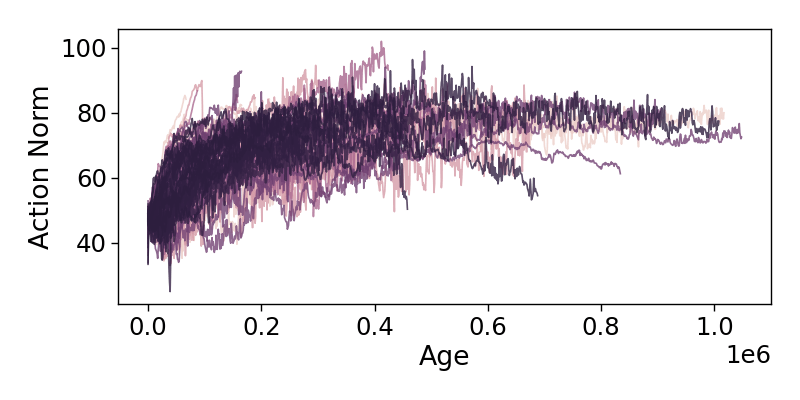
\includegraphics[width=7cm]{actnorm_age-min.png}
  \end{subfigure}
  \caption{Change of the average action norm over aging for highly active and productive agents in \texttt{x2 Active Metabolism}. Specifically, agents with more than $60$ average action norm and more than $10$ children are selected for visualization.}\label{figure:actnorm-age}
\end{figure}

To investigate the reason, we plot the relationship between the average of action norm ($|a_{t}^{i}|$) over agents' lifetime and the number of children in the right of \cref{figure:scatter-metabo}. As shown in the left of \cref{figure:scatter-metabo}, agents in the \texttt{x2 Active Metabolism} setting consume less energy when the action norm is less than $50$, but they consume more energy otherwise. In both settings, agents with roughly $30$ to $60$ average action norms produce more children. Surprisingly, we can see that agents with more than $50$ average action norms produce more children in the \texttt{x2 Active Metabolism} setting, although their energy consumption is higher. However, as shown in \cref{figure:actnorm-age}, agents tend to take smaller actions in their early stage of learning. Thus, we can say that doubling active metabolism is milder than doubling basic metabolism because it's not that harsh for newborns, leading to smaller action rewards.

\begin{figure}[t]
  \begin{subfigure}[t]{4cm}
    \centering
    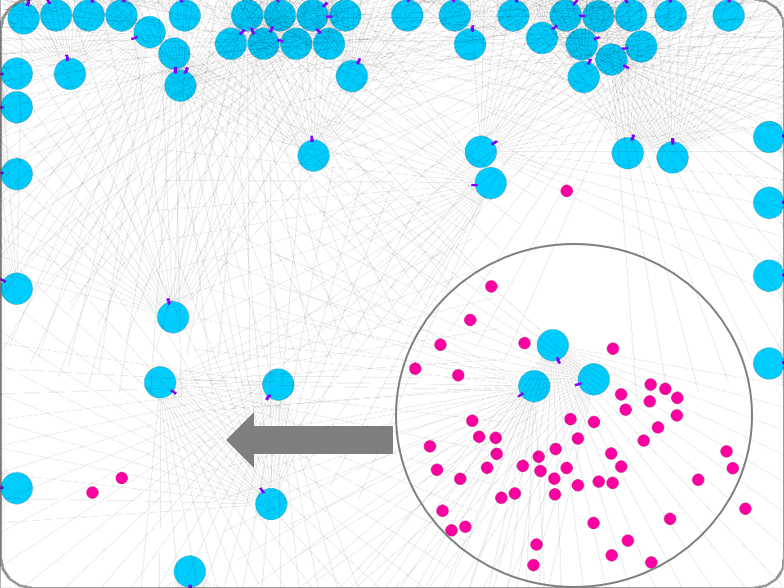
\includegraphics[width=4cm]{moving-annot-min.png}
  \end{subfigure}
  \begin{subfigure}[t]{4cm}
    \centering
    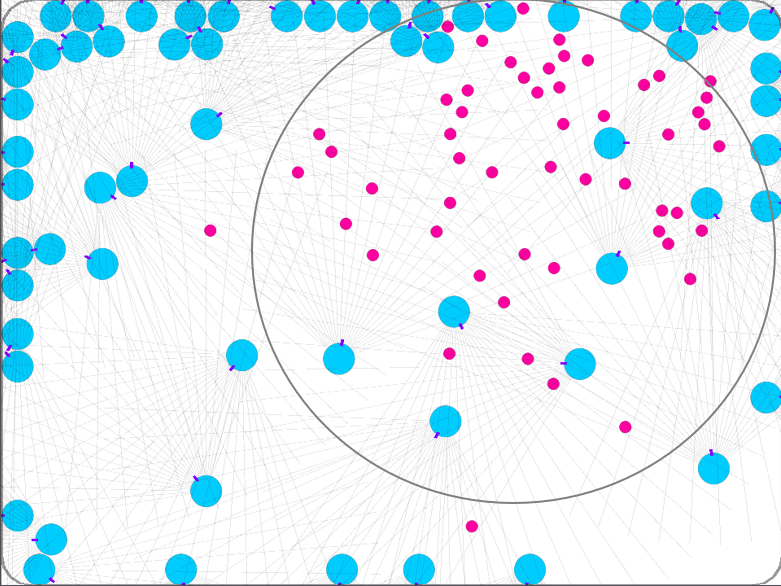
\includegraphics[width=4cm]{lv-annot-min.png}
  \end{subfigure}
  \caption{
    \textbf{Left:} Environment with food relocation.
    \textbf{Right:} Environment with spread foods.
  }\label{figure:foodloc}
\end{figure}

\begin{figure}[ht]
  \centering
  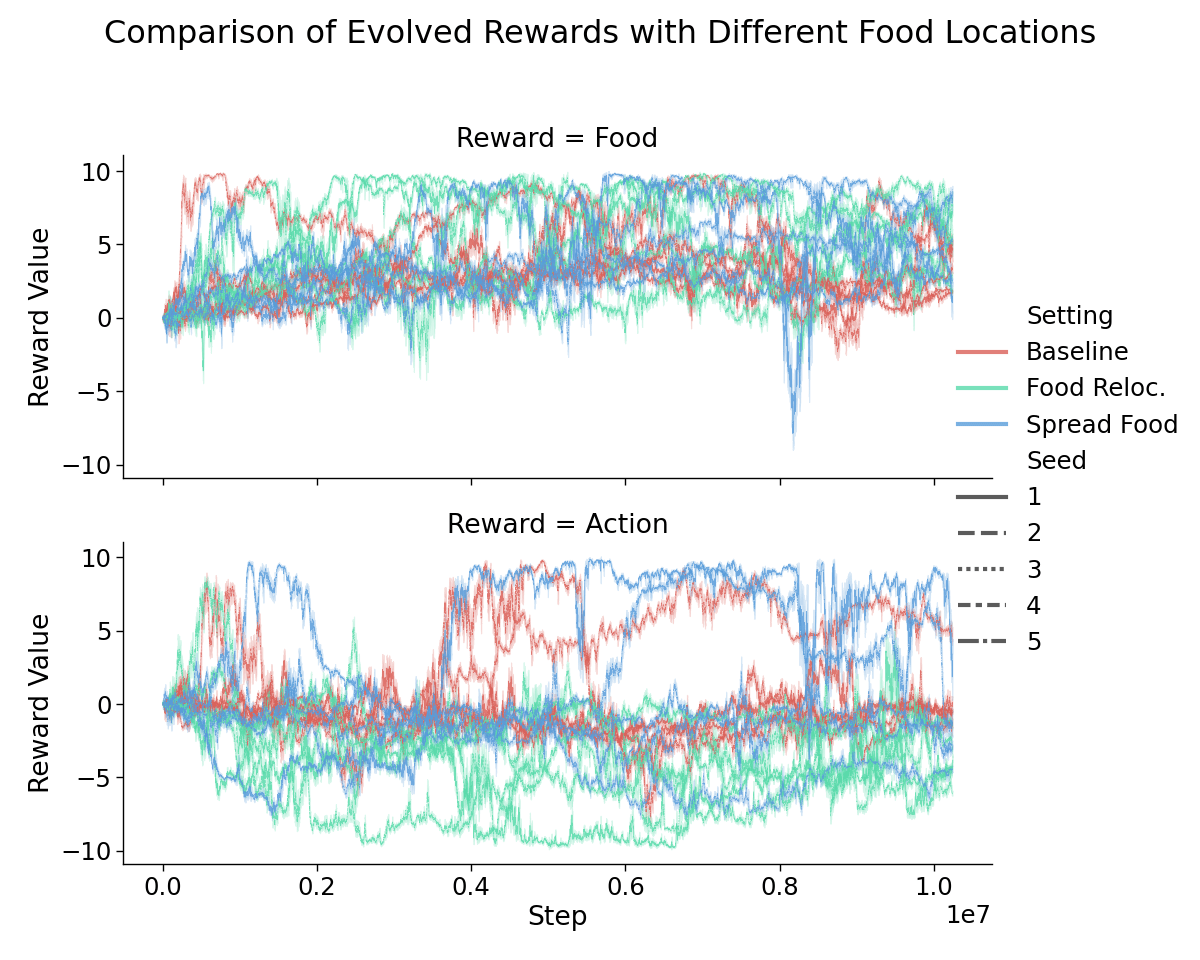
\includegraphics[width=8cm]{comp_foodloc-min.png}
  \caption{
    Comparison of evolved rewards between different food locations.
  }\label{figure:result-foodloc}
\end{figure}

\begin{figure}[!htb]
  \centering
  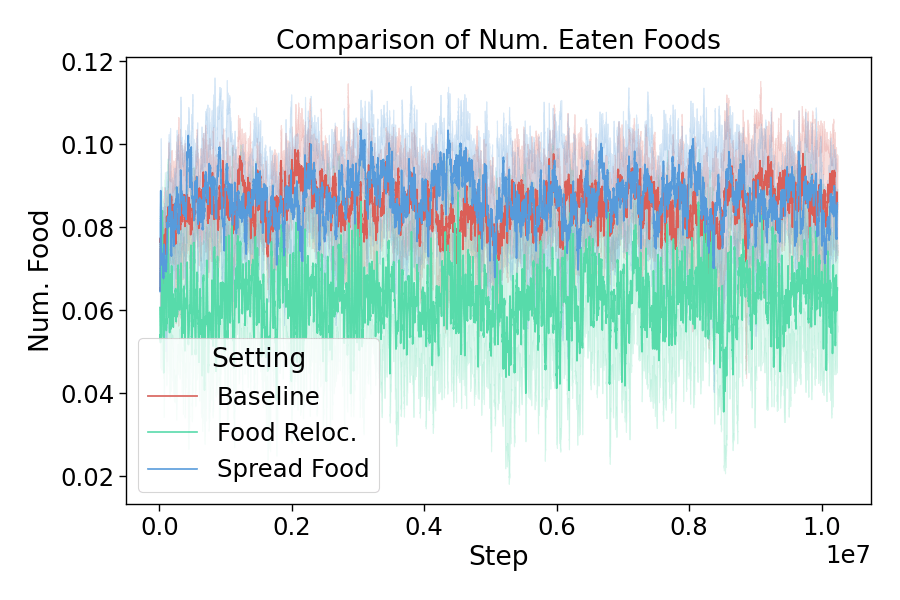
\includegraphics[width=8cm]{comp-nfoods-min.png}
  \caption{
    Comparison of the average number of foods that agents ate between different food locations.
    Rolling mean over 10000 steps is taken for clear visualization.
  }\label{figure:result-ncstd}
\end{figure}

\paragraph{Effect of Food Location}
In the baseline setting, the center of the food location is a fixed location with a small variance, which can make the agents less active. The penalty for motor action can be smaller in the environment where agents need to hunt foods more actively. To confirm this hypothesis, we compare the evolved rewards in the baseline environment with ones in the environment where the food relocation happens clockwise (\texttt{Food Reloc.}) and the environment with more spread foods (\texttt{Spread Food}) shown in \cref{figure:foodloc}. Note that in the food repositioning setting, the center of food reproduction moves slightly clockwise after 100 foods are eaten. We show the results in \cref{figure:result-foodloc}. As our hypothesis suggests, action rewards are more likely to be positive in the spread food setting. However, contradicting our hypothesis, action rewards tend to be more negative in the food reloaction.

To explore the reason, we plot the standard deviation of the number of children in the group of agents alive at a certain time step in \cref{figure:result-ncstd}. While the standard deviation is often quite high in the baseline and \texttt{Spread Food} setting, it's constantly low in the \texttt{Food Reloc.} setting.

\paragraph{Effect of Poor and Poisonous Foods}

\begin{figure}[t]
  \begin{subfigure}[t]{4cm}
    \centering
    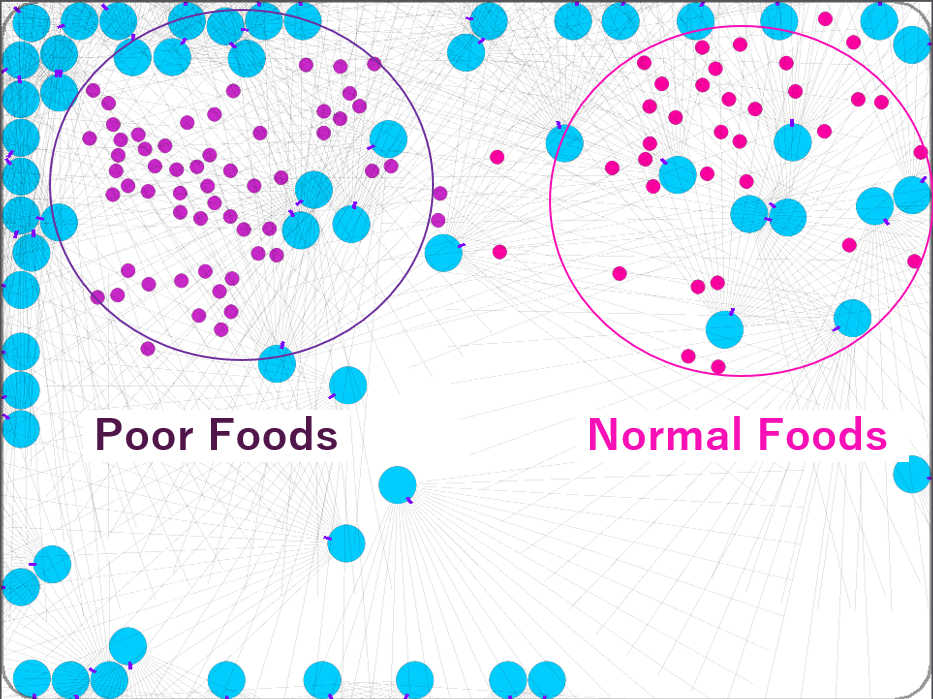
\includegraphics[width=4cm]{poor-annot-min.png}
  \end{subfigure}
  \begin{subfigure}[t]{4cm}
    \centering
    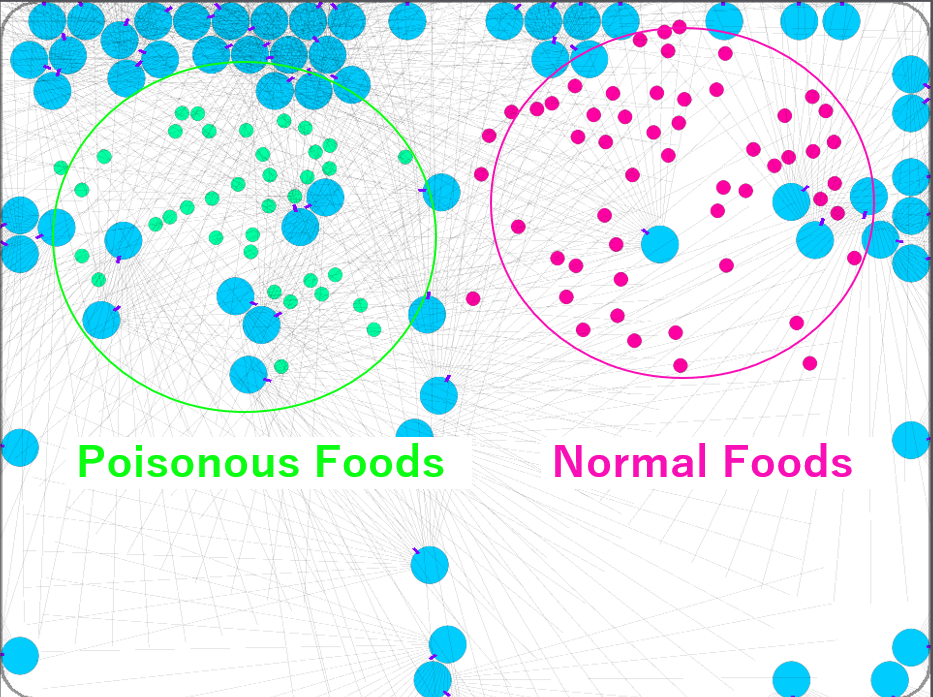
\includegraphics[width=4cm]{poison-annot-min.png}
  \end{subfigure}
  \caption{
    \textbf{Left:} Environment with poor foods.
    \textbf{Right:} Environment with poisonous foods.
  }\label{figure:pp}
\end{figure}

\begin{table}[t]
  \begin{subtable}[h]{0.45\columnwidth}
    \centering
    \begin{tabular}{cc}
      \toprule
      Parameter & Value \\
      \midrule
      $n_{\textrm{max}}^{\textrm{normal}}$ & 40\\
      $g^{\textrm{normal}}$ & 0.01 \\
      $n_{\textrm{max}}^{\textrm{poor}}$ & 60 \\
      $g^{\textrm{poor}}$ & 0.02 \\
      \bottomrule
    \end{tabular}
  \end{subtable}
  \begin{subtable}[h]{0.45\columnwidth}
    \centering
    \begin{tabular}{cc}
      \toprule
      Parameter & Value \\
      \midrule
      $n_{\textrm{max}}^{\textrm{normal}}$ & 60\\
      $g^{\textrm{normal}}$ & 0.01 \\
      $n_{\textrm{max}}^{\textrm{poison}}$ & 40 \\
      $g^{\textrm{poison}}$ & 0.01 \\
      \bottomrule
    \end{tabular}
  \end{subtable}
  \caption{
    Food regeneration parameters with poor foods (left) or poisonous foods (right).
    $n_{\textrm{max}}^{\textrm{poor}}$ and $n_{\textrm{max}}^{\textrm{poison}}$ are the maximum number of poor or poisonous foods, while $g^{\textrm{poor}}$ and $g^{\textrm{poison}}$ are growth rate of poor or poisonous foods.
  }\label{table:pp}
\end{table}

In the experiments so far, there is only one kind of food with $e_{\mathrm{food}} = 1.0$ in the environment. However, one role of our reward system is to distinguish between different external stimuli. For example, our food reward system helps us eat nutritious food, avoiding poisonous foods. Therefore, we conduct simulations with poor and poisonous foods, of which the energy gains are $e_{\mathrm{poor}} = 0.2$ and $e_{\mathrm{poison}} = -0.4$. In \cref{figure:pp}, we show environments with poor and poisonous rewards. In those environments, we fix the center of poor or poisonous food location at the upper left. The number of maximum foods is smaller in the environment with poor foods, and there are more normal foods in the environment with poisonous foods as shown in \cref{table:pp}, so that the overall energy supply should be roughly the same.

\begin{figure}[t]
  \centering
  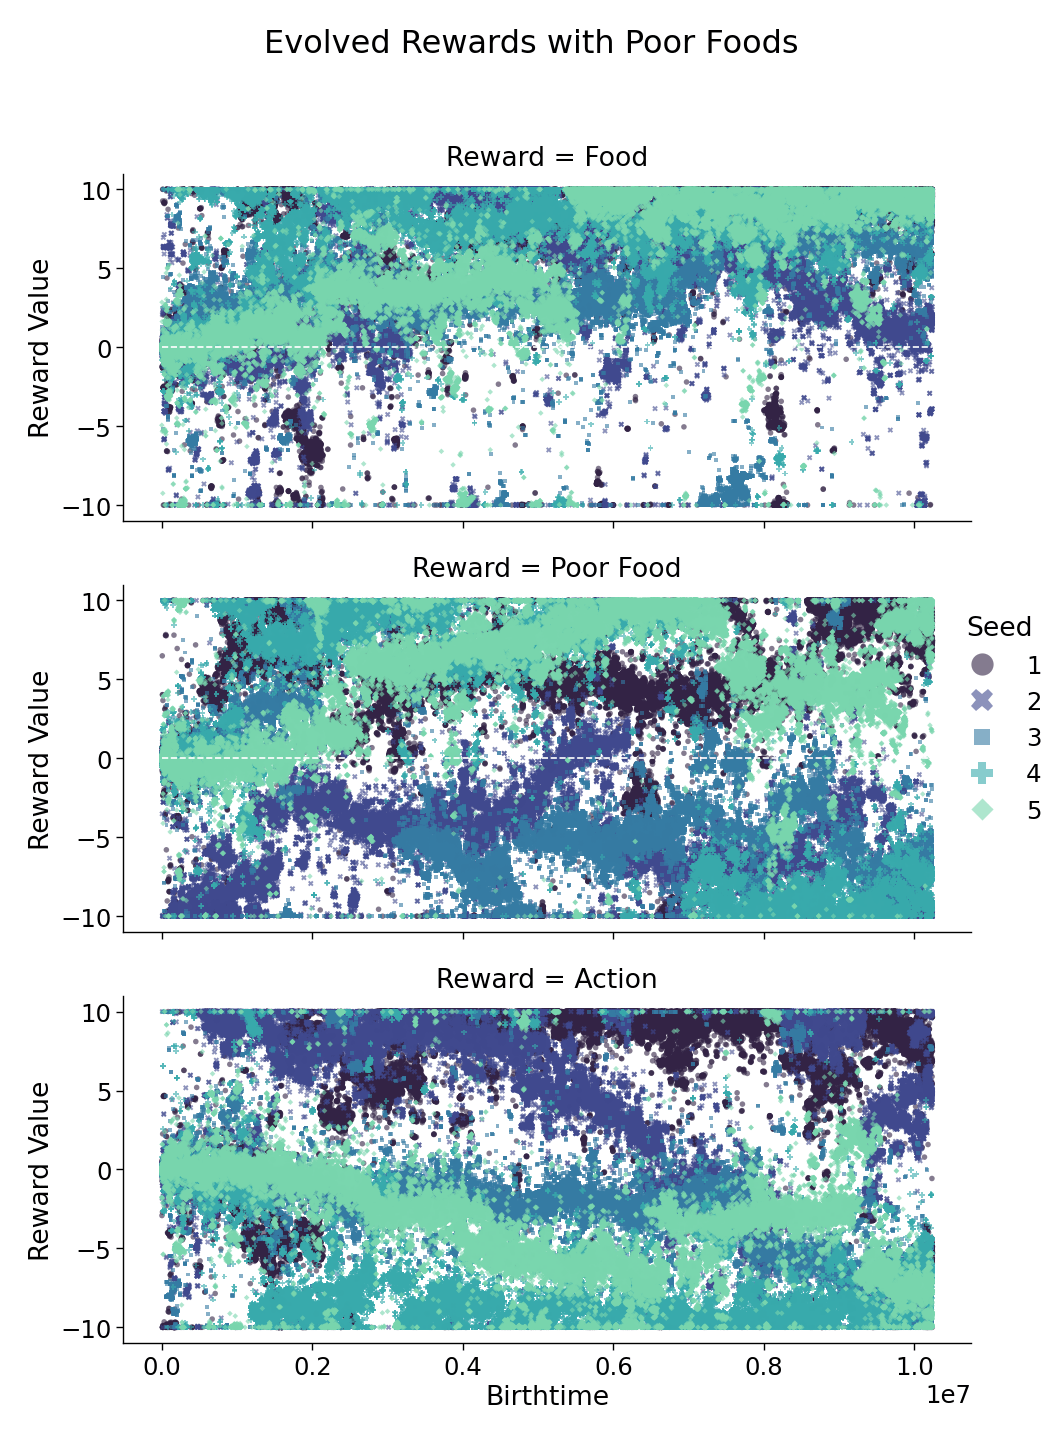
\includegraphics[width=8cm]{poor-min.png}
  \caption{
    Evolved rewards with poor foods.
    From top to bottom, we show rewards for normal foods, poor foods, and action.
  }\label{figure:result-poor}
\end{figure}

\begin{figure}[!htb]
  \centering
  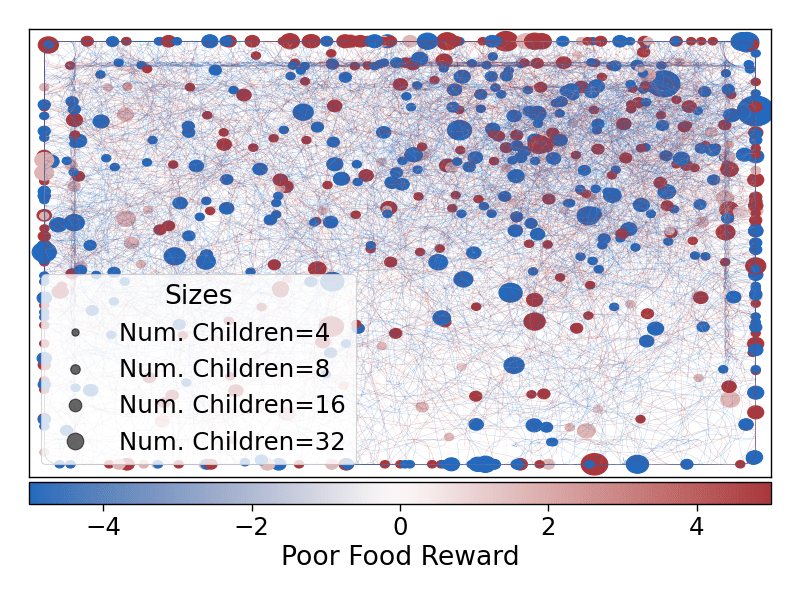
\includegraphics[width=8cm]{lh-f2-min.png}
  \caption{
    The life history of agents in the environment with poor foods.
    Lines indicate the trajectories and the circle indicates places where agents got their children.
    The circle's radius corresponds to the number of grandchildren that the newborn produced.
  }\label{figure:lh-poor}
\end{figure}

\begin{figure}[!htb]
  \centering
  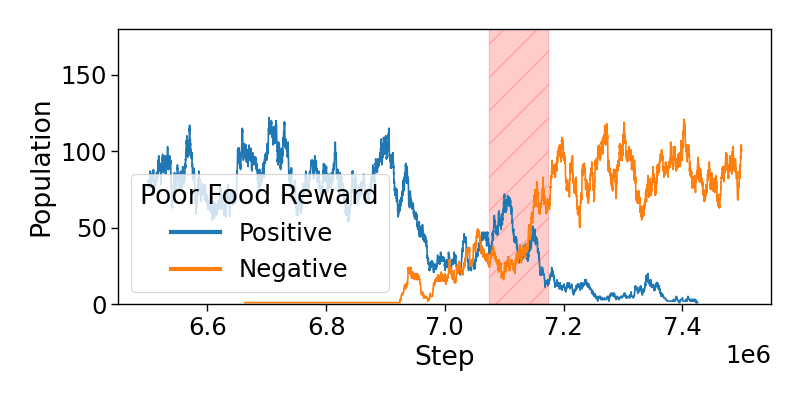
\includegraphics[width=8cm]{popc-poor-min.png}
  \caption{
    The population of agents with positive or negative rewards for poor foods.
    The area filled in red shows the time period corresponding to \cref{figure:lh-poor}.
  }\label{figure:pop-poor}
\end{figure}

\Cref{figure:result-poor} shows the results with poor foods. While rewards for normal foods are consistently positive in all five runs, the evolution of rewards for poor foods is unstable. In \cref{figure:lh-poor}, we show the life history of agents in a selected period with almost equal number of agents with positive or negative food rewards (seed $4$, step $\num{7.1e6}$ to $\num{7.2e6}$). Lines indicate the trajectories and the circle indicates places where agents got their children. The size of the circles corresponds to the number of grandchildren that the child born in that place made, indicating the influence of the reproduction event. In this period, agents with negative rewards for poor foods tend to produce many children in the right area of the environment with normal foods, leading to a population increase. This case study shows that avoiding poor foods can lead to eating more nutritious foods in this environment. At the same time, eating poor foods is not harmful to agents, leading to a very unstable evolution of rewards for poor foods.

\begin{figure}[!ht]
  \centering
  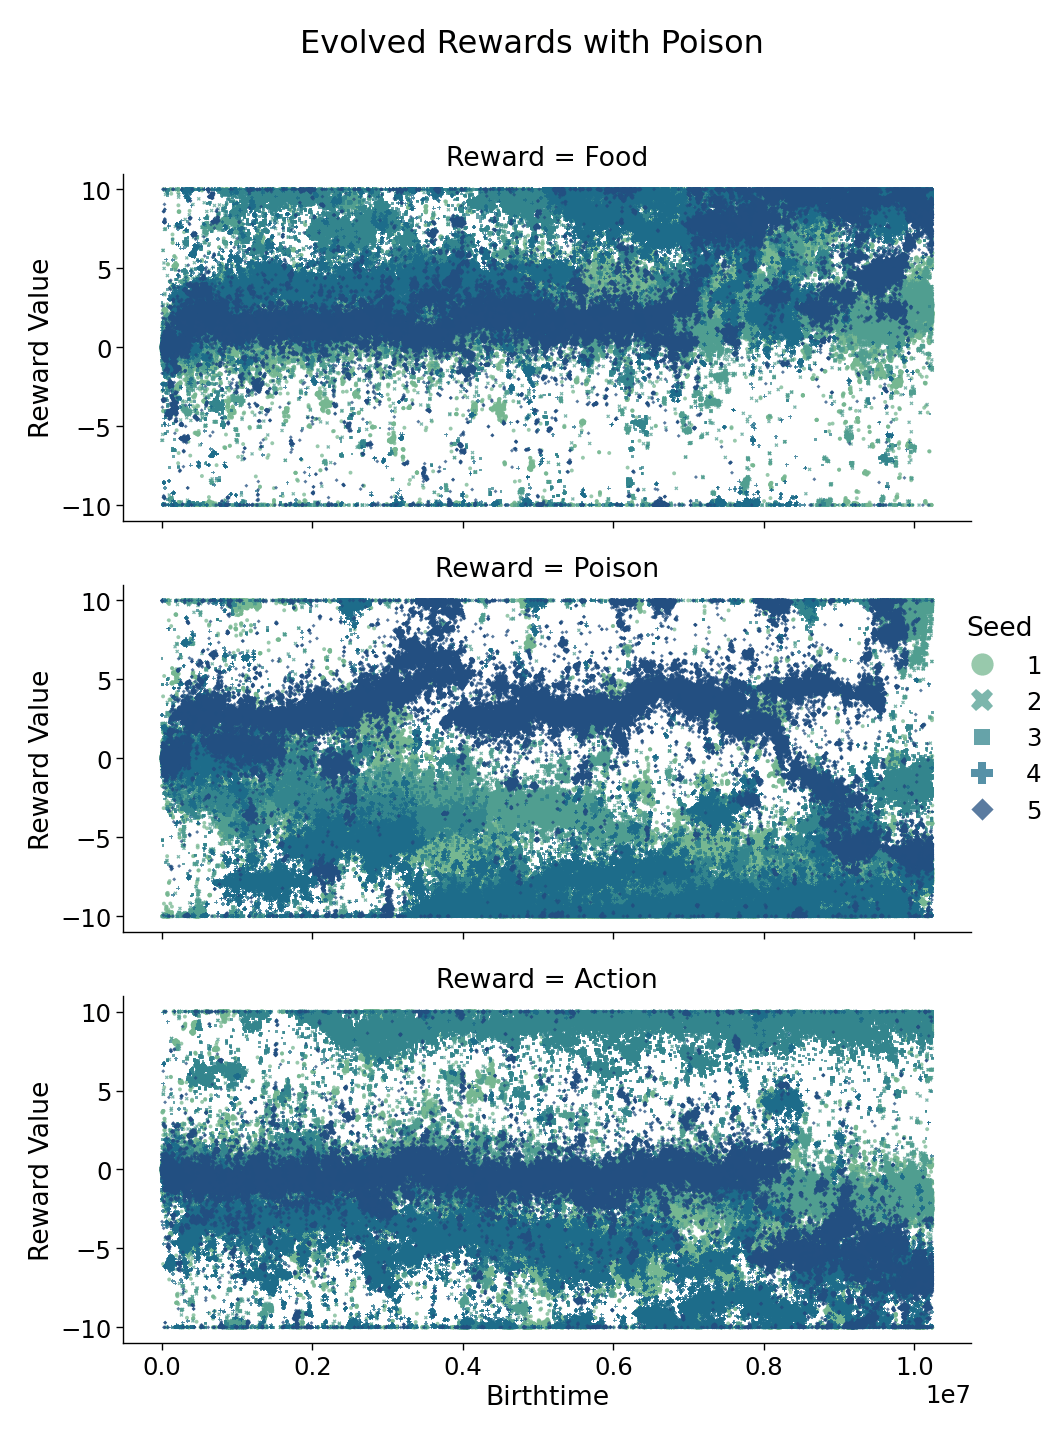
\includegraphics[width=8cm]{poison-min.png}
  \caption{
    Evolved rewards with poisonous foods.
    From top to bottom, we show rewards for normal foods, poisonous foods, and action.
  }\label{figure:result-poison}
\end{figure}

\begin{figure}[!htb]
  \centering
  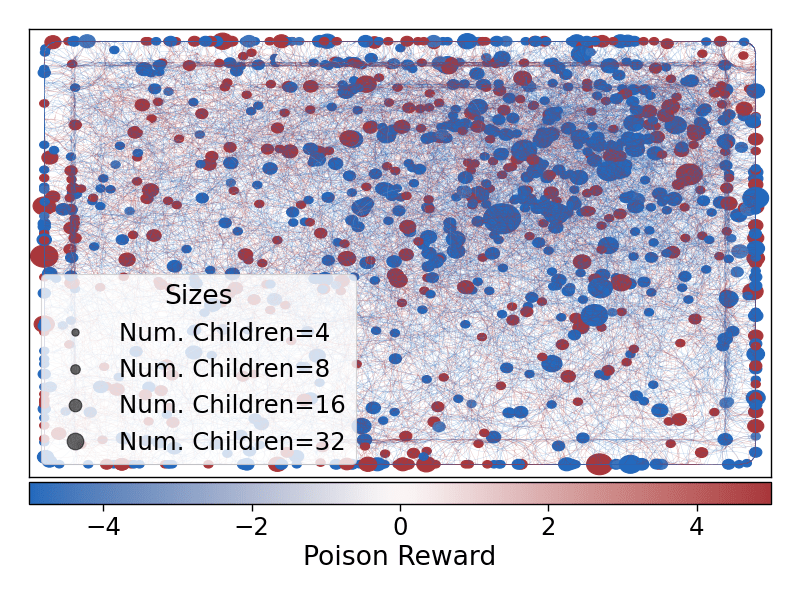
\includegraphics[width=8cm]{lh-poison2-min.png}
  \caption{
    The life history of agents in the environment with poisonous foods.
    Lines indicate the trajectories and the circle indicates places where agents got their children.
    The radius of the circle corresponds to the number of grandchildren that the newborn produced.
  }\label{figure:lh-poison}
\end{figure}

\begin{figure}[!htb]
  \centering
  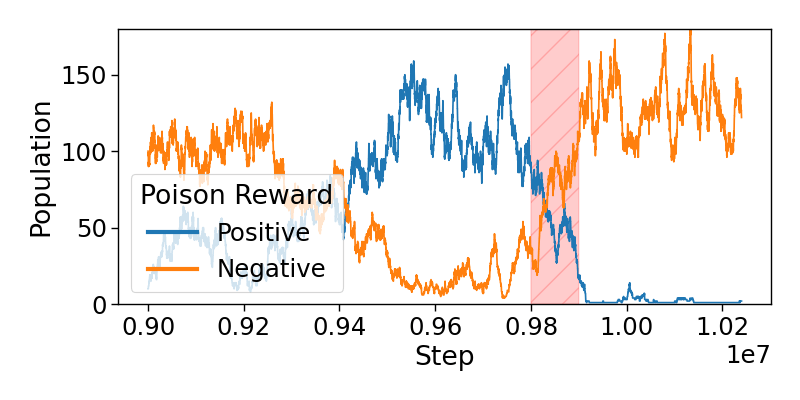
\includegraphics[width=8cm]{popc-poison-min.png}
  \caption{
    The population of agents with positive or negative rewards for poor foods.
    The area filled in red shows the time period corresponding to \cref{figure:lh-poison}.
  }\label{figure:pop-poison}
\end{figure}

\Cref{figure:result-poison} shows the results with poisonous foods. Like the case with poor foods, rewards for normal foods are positive in all runs. The rewards for poisonous foods are consistently negative in most runs, as expected. Although in seed $5$ agents with positive poison rewards are dominant for a long time, eventually agents with negative poison rewards branch and replace them, as shown in \cref{figure:pop-poison}. In \cref{figure:lh-poison}, we plot the agent's trajectory and reproduction record during this transition period (step $\num{9.8e6}$ to $\num{9.9e6}$) marked red in \cref{figure:pop-poison}.

\section{Conclusion}
In this paper, we propose a distributed evolutionary simulation to investigate the evolution of reward function.